\chapter{Introduction}
\label{chap:introduction}
\section{Motivation and Background}
As the world strives towards greener energy, different renewable energy alternatives are being explored. Wind energy has been utilized by man for over thousands of years, and in the recent years become one of the more mature renewable energies. As the areas on land that are fit for wind turbines are scarce, and the public is disliking the noise and visibility of the wind turbines, technology is pushing towards offshore wind parks. Moving the wind parks offshore is not only solving the problems with complaints from the public, but wind speed tends to increase with distance from shore. In the last years, there has been an increase in scale, capacity and distance from shore each year for offshore wind installations. Moving further from shore often implies moving into deeper waters, making floating wind turbines the most plausible technology. Floating wind turbines are similar to semi-submersible oil platforms, but will have very different motions, as geometry and wind loads are significantly different. A lot of research has been done in terms of estimating the lifetime for flexible risers and umbilicals in relations to fatigue for the oil and gas industry. For floating wind turbines, there is significantly less research done in terms of the lifetime of dynamic flexible cables. The power cable technology and the lifetime of power cables are some of the most important limiting factors of moving wind floating wind turbines further away from the shore and into deeper waters. Research is needed in order to continue the development of floating wind turbines in the future, \cite{Thies2012}. \newline
\newline
Lifes50+ is a project financed by the Horizon2020 program where the goal is to develop cost-effective floating solutions for 10MW wind turbines, \cite{Horizon2010}. The project consists of 4 different designs and 3 different locations. One of the designs in the project is the OO-Star developed by Dr. Techn. Olav Olsen shown in Figure \ref{fig:oostarintro}. This was considered an appropriate case study to investigate the lifetime of dynamic power cables further. 

\begin{figure}[H]
\centering
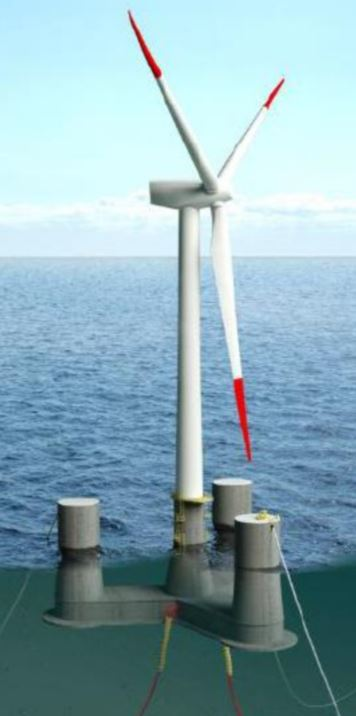
\includegraphics[scale=0.5]{figures/oostar}
\caption[$\; \:$Dr. Techn. Olav Olsen's OO-Star]{Dr. Techn. Olav Olsen's OO-Star \cite{Lifes50+D4.2} }
 \label{fig:oostarintro}
\end{figure}


\section{Literature Review}
A literature search was done prior to the project thesis. \cite{Feld1995} looked at the applied loads and responses of the metallic elements for subsea configurations. \cite{Chien2004} discussed different cable designs for 250MW offshore power transmission and concluded that they do not behave like umbilicals dynamically, and that harmonics do occur during transmission. \cite{Karlsen2010} presented a test method for simulating fatigue of a dynamic power cable that included the effects of fretting, creep and friction. \cite{Nasution2013} investigated fatigue on 95mm$^2$ copper conductors experimentally and by the use of FEM. Single wires from different layers were tested in tension and the full cross-section was tested in bending. The full cross-section showed lower fatigue strength that the individual wires and trellis points were particularly vulnerable, as cracks initiated from these points. It was suggested that the difference in results between the testing and the FEM analyses was due to the surface irregularities in the wires from the packaging of the conductor. \cite{NASUTION2014} did similar tests and concluded that all first fatigue failures in tension-tension of the full cross-section happened in the outer layers of the conductors, in the thinnest parts of the wires, that is, the trellis points. For tension-bending mode, all the failures occurred in the inner layer of the conductor. It was concluded that this indicated that the effect of friction between layers plays an important role in the lifetime of the cross-section. The report also comments that as the longitudinal stress governs the fatigue performance, beam elements can be used with good results in analyses. \cite{savik2014} did experimental and FEM analysis of fatigue strength with 300mm$^2$ conductors. This study concluded with that in terms of maximum stress, individual wires from 95mm$^2$  and 300mm$^2$ wires fall in a common scatter band, and that lubricated conductors have longer fatigue life than unlubricated conductors. The study also supports the previous conclusions that crack initiation starts from trellis points. In this article, an analytic method to calculate the stress variation in the individual wires of the conductor was developed. \cite{Taninok2017} looked at dynamic cable systems for 2MW and 100kW floating offshore wind installations and concluded that their proposed cable profile absorbed the floater behavior so that there was no motion in the cable at the bottom hang off.  

\section{State of the Art}
\subsection{Offshore Wind Turbines}
According to ISSC 2018 committee V.4: OFFSHORE RENEWABLE ENERGY: (\cite{Gao2018}): "Offshore wind is by far the most developed technology and
promising cost reduction has been achieved in the last few years", in terms of offshore renewable technologies. Figure \ref{fig:sit17} shows the development of offshore wind capacity until 2017. 

\begin{figure}[H]
\centering
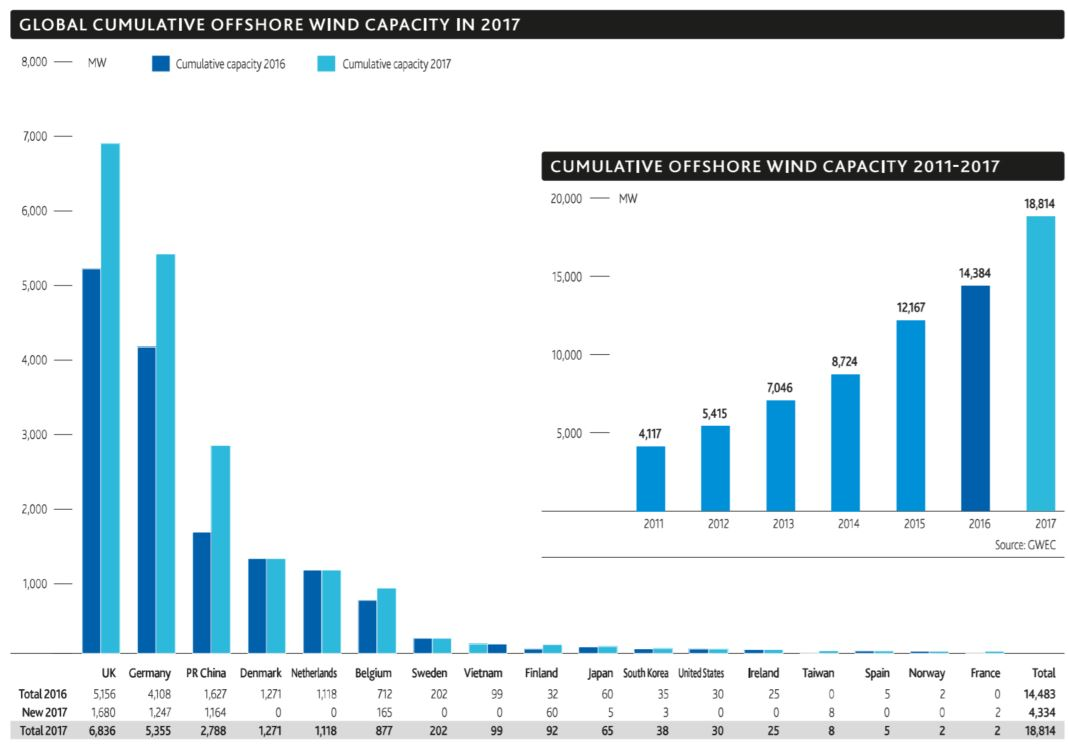
\includegraphics[scale=0.8]{figures/sit17}
\caption[$\; \:$Cumulative Offshore Wind Capacity in 2017]{Cumulative Offshore Wind Capacity in 2017 \cite{GWEC2018}}
 \label{fig:sit17}
\end{figure}

\noindent The majority of the offshore wind farms are located in Europe. Figure \ref{fig:world} shows the current market situation of offshore floating wind turbines. As can be seen, it is mainly Europe, USA, and China that are represented. 


\begin{figure}[H]
\centering
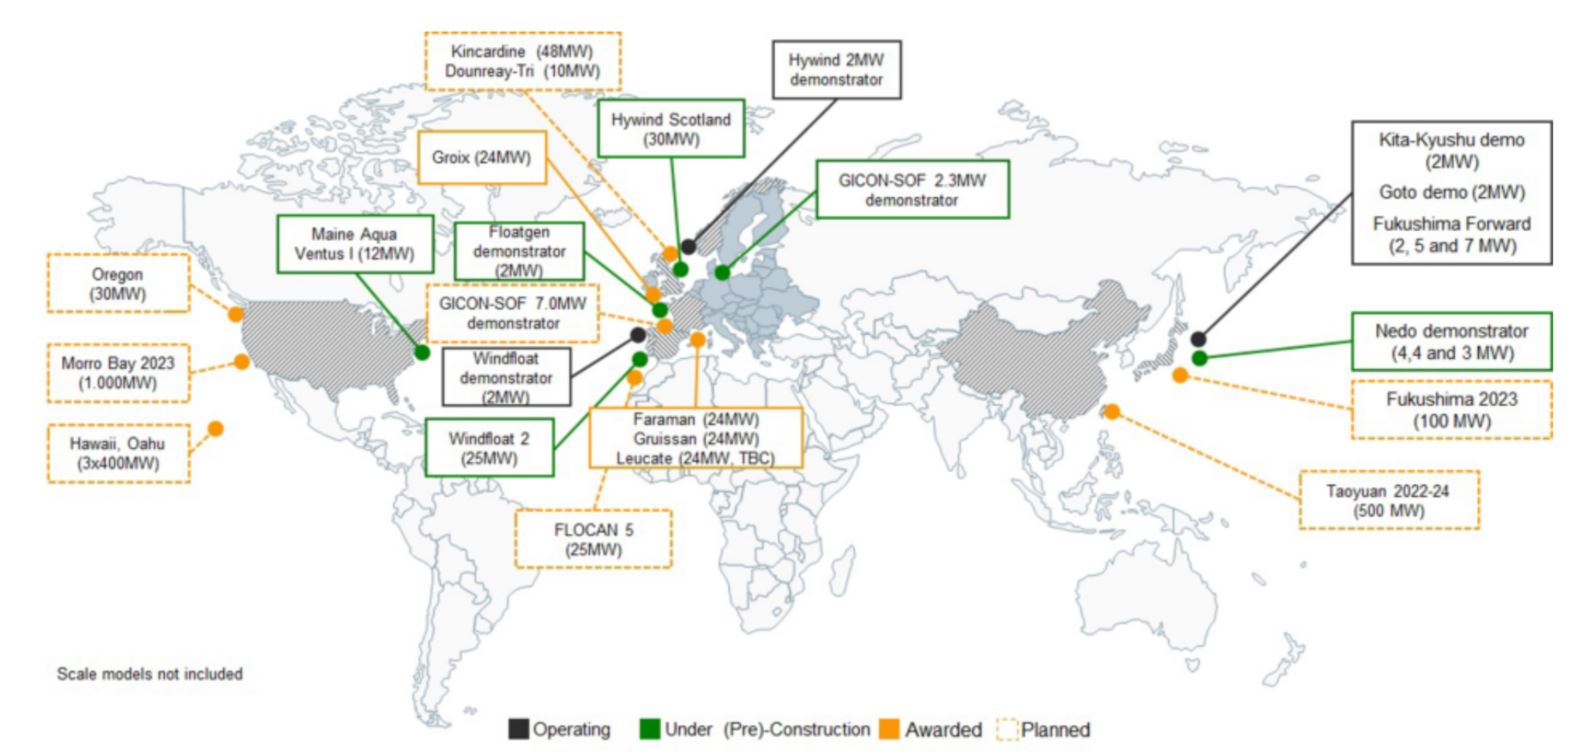
\includegraphics[scale=0.54]{figures/world}
\caption[$\; \:$Current market situation of offshore floating wind turbines]{Current market situation of offshore floating wind turbines \cite{Gao2018}}
 \label{fig:world}
\end{figure}

\noindent In the recent years, installations have moved further from shore, into deeper waters and with large farm configurations and larger turbines.  Longer blades will give advantages in terms of overall cost, but also challenges for installation, \cite{Gao2018}.  Figure \ref{fig:diameter} shows the development of power capacity for the last two centuries. The average size in 2017 was 5.9 MW. That is an increase of 23\% from 2016 according to \cite{we2018}.

\begin{figure}[H]
\centering
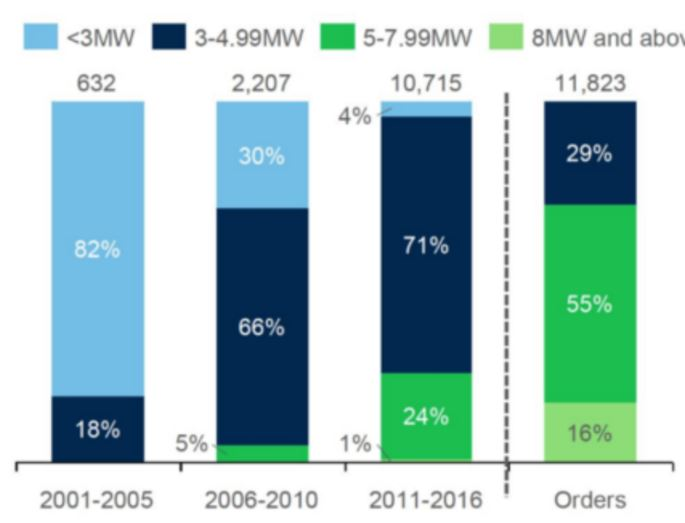
\includegraphics[scale=0.7]{figures/diameter}
\caption[$\; \:$Development of turbine size]{Development of turbine size. \cite{Deigen2018}}
 \label{fig:diameter}
\end{figure}

 \noindent In 2016, the first 8 MW turbine was installed in the Irish Sea in the UK. In Norway, Statoil made a step towards commercialization of floating wind farms by installing the first floating wind farm with 5 6MW spar wind turbines called Hywind, outside of Scotland. Hywind can be used at depths up to 800m, and enable offshore wind energy installations for areas that have been unavailable until now \cite{Equinor2018}. Short-term plans for the offshore wind industry include the installation of two small floating wind farms in the US as well as prototype testing for exiting prototypes in Norway, Portugal, and Japan, and planned prototype development in Japan, France, and Germany.  Two large wind farms are planned on the east coast of the US, one 120 MW farm outside of Maryland, and one 90 MW on the coast of New York. \cite{Gao2018}. \newline
 \newline
 \cite{Bailey2014} states that "Commercialization of floating wind farms is
anticipated between 2020 and 2025." In 2014 the European Union set a legally binding target that 27\% of the energy consumption are to come from renewable energy sources in 2030. \cite{EWEA2015}  presents three different scenarios on the development of offshore wind energy by 2030, and in the central scenario, it is suggested that 66 GW come from offshore wind. To achieve this goal, there needs to be an annual average increase of 15\%. \cite{Gao2018} states that this is probably possible as we have seen an increase of 25\%-30\% annually the recent years. US Department of Energy has a goal of 86 GW of energy provided from offshore wind by 2050. \cite{windus2016}. 
\subsection{Power Cables}
The trend over the years has been that offshore wind installations move further away from shore. This development can be seen in Figure \ref{fig:distshore}. 

\begin{figure}[H]
\centering
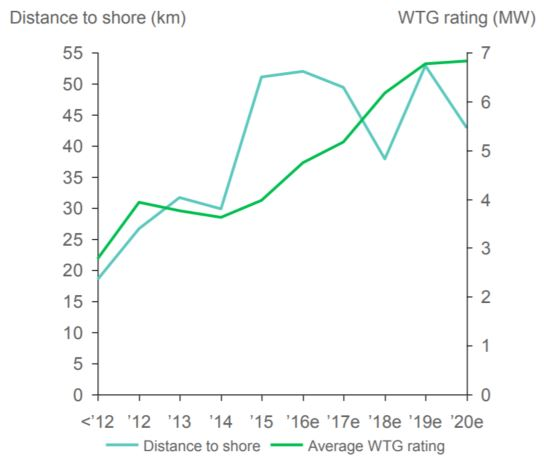
\includegraphics[scale=0.9]{figures/distshore}
\caption[$\; \:$Distance to shore ]{How distance to shore have increased in recent years \cite{Make2016}}
 \label{fig:distshore}
\end{figure}

\noindent \cite{srinil2016} states that traditionally, the w shape configuration has been used for inter-array cabling, and the lazy wave has been used for export cables, see Figure \ref{fig:cableconfig}. However, according to \cite{ds2010}, the lazy wave configuration is being considered for inter-array in newer projects such as the Statoil's Hywind project, and the Fukushima Floating Offshore Wind
Farm Demonstration Project, \cite{yagihashi2015dynamic}. Inter-array cables are usually three-core copper conductors, armoured with steel wires with insulation around the conductors. 33kV is usually the standard for offshore cables, however, 66kV are under development \cite{srinil2016}. 


\begin{figure}[H]
\subfloat[Traditional W-shape for inter array cable \label{fig:dc}]
  {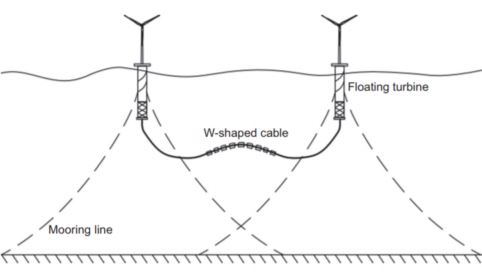
\includegraphics[width=.45\linewidth]{figures/wshape}}\hfill
\subfloat[Lazy wave shape, traditionally only used for export cables \label{fig:ac}]
  {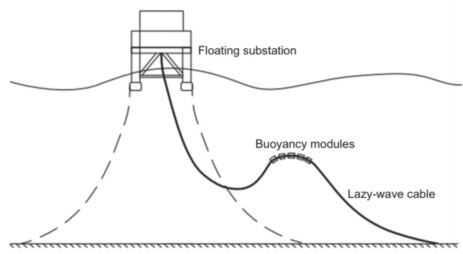
\includegraphics[width=.45\linewidth]{figures/lw}}\hfill
\caption[$\; \:$Cable configurations]{Different cable configurations, \cite{ds2010}}
\label{fig:cableconfig}
\end{figure}

\section{Objective}
The objective of this Master Thesis is to estimate the lifetime of a dynamic power cable applied in offshore wind farms. Theory and software used and developed for the oil and gas industry, is applied in the relatively new and upcoming field of ocean renewable energy.

A Project Thesis was executed in the fall of 2018 lays the basis for this Master Thesis where a local and a global model were modelled                 ....

This is achieved by performing a local and a global analysis on a selected wind turbine floater at a selected location. The global analysis is executed first in SIMA RIFLEX on a global model consisting of the total cable attach to the sea floor and to the vessel. A scatter diagram for the wave conditions at the selected location is used, and all the different sea states (i.e. the different combinations of Hs and Tp) are analyzed for one hour each in the global analysis. The output of the global analyses are time series of the angle between the vessel and the cable, and tension in the cable hang off. The cycles of the time series are counted using rain-flow counting implemented in Python, and result in histograms with the number of cycles for each angle scaled for occurrence in the scatter diagram.  This will be used as input in the local analyses.\\\\ The local analyses is be performed in BFLEX, and the local model consists the top of the cable where the fatigue damage will be most severe. Each angle range is analyzed for one cycle with the corresponding tension level found by linear interpolation. From this, the stress variation in each individual wire in the copper conductor is calculated, and the total damage pr year is found using  and SN fatigue data and Miner-Palmgren formula will be used to estimate the lifetime of the dynamic power cable. \\\\ The objective of this report is, therefore, to conduct a literature study, acquire the necessary theoretical background, select an appropriate case study and create the models that will be used in the master thesis. All choices and simplifications are to be described and justified. 

\section{Project Thesis Structure}
\begin{itemize}
    \item Chapter 1 contains the introduction with literature review, state of the art and objective for the project thesis.
     \item Chapter 2 is the system theory for wind turbines, offshore wind turbines and power cables.
      \item Chapter 3 goes through the basic theory of wave-induced fatigue. 
      \item The case scenario that will be investigated is presented in Chapter 4
      \item Chapter 5 describes the theory behind the two numeric models
      \item In chapter 6, the modeling methodology will be explained.
      \item 
      \item
\end{itemize}
\section{Contribution}


\section{Master Thesis Structure}

